\section{ارزیابی عملکرد مدل}
\label{sec:evaluation}

در این بخش، عملکرد مدل آموزش‌دیده روی داده‌های آزمون ارزیابی می‌شود. ابتدا پیش‌بینی‌های مدل با مقادیر واقعی مقایسه شده و سپس با استفاده از معیارهای ارزیابی، دقت مدل بررسی می‌شود.

\subsection{پیش‌بینی روی داده‌های آزمون}

از مدل آموزش‌دیده برای پیش‌بینی عمر باقی‌مانده باتری‌ها در مجموعه آزمون استفاده می‌شود. از آنجا که مقادیر هدف در مرحله آموزش به بازه ۰ تا ۱ نرمال‌سازی شده‌اند، برای بازگرداندن پیش‌بینی‌ها به مقیاس اصلی، مقادیر خروجی در ۲۰۰۰ ضرب می‌شوند.

با در اختیار داشتن مقادیر واقعی و پیش‌بینی‌شده، نموداری برای مقایسه این دو مقدار رسم می‌شود. در حالت ایده‌آل، نقاط داده باید بر نیمساز ربع اول و سوم منطبق باشند یا دست‌کم در نواری باریک پیرامون آن قرار گیرند. بااین‌حال، نمودار حاصل پراکندگی بیشتری را نشان می‌دهد و شامل پنج روند مجزا، متناظر با پنج باتری مجموعه آزمون است. این مقایسه در شکل~\ref{fig:scatter} ارائه شده است؛ محور افقی مقدار واقعی RUL و محور عمودی مقدار پیش‌بینی‌شده را نشان می‌دهد و خط مرجع، حالت برابری این دو مقدار را مشخص می‌کند.

\begin{figure}[!htbp]
\centering
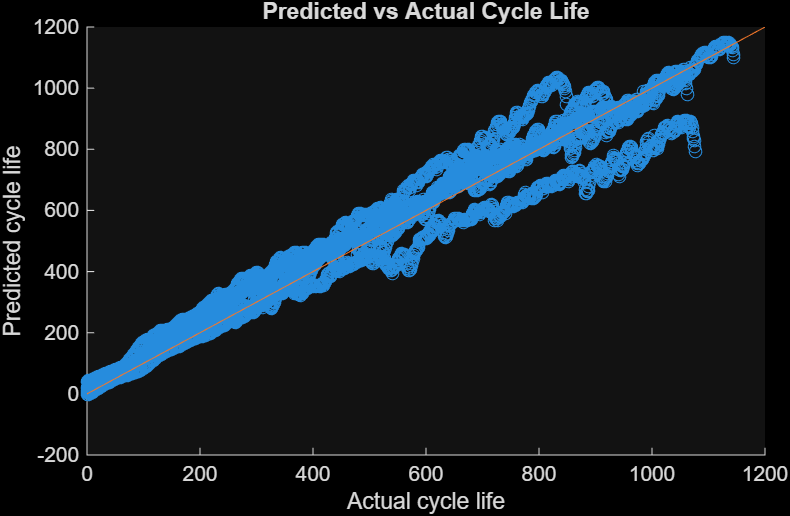
\includegraphics[width=0.8\textwidth]{img/scatter.png}
\caption{مقایسه مقدار واقعی و مقدار پیش‌بینی‌شده RUL برای پنج باتری مجموعه آزمون؛ خط مورب، حالت برابری مقدار واقعی و پیش‌بینی‌شده را نشان می‌دهد.}
\label{fig:scatter}
\end{figure}

در نمودار مشاهده می‌شود که با نزدیک‌شدن مقدار واقعی عمر باقی‌مانده به صفر، نقاط هر پنج باتری نیز به ناحیه نزدیک مبدأ و خط مرجع نزدیک می‌شوند. این الگو با کاهش خطای مطلق پیش‌بینی در مقادیر پایین RUL سازگار است؛ بااین‌حال، صرفاً بر اساس این نمودار نمی‌توان درباره کاهش قطعی عدم‌قطعیت پیش‌بینی نتیجه‌گیری کرد.

برای بهبود نتایج، پیشنهاد شده است که مدل با استفاده از مجموعه‌داده‌ای بزرگ‌تر و غنی‌تر آموزش داده شود و تنظیم ابرپارامترهای آن نیز مورد بررسی قرار گیرد.

\subsection{معیارهای ارزیابی}

در نهایت، عملکرد مدل با استفاده از دو معیار و بر اساس داده‌های مجموعه آزمون ارزیابی می‌شود. معیارهای \lr{RMSE} و \lr{MAE} که تعریف آن‌ها به‌ترتیب در روابط~\eqref{eq:rmse} و~\eqref{eq:mae} آمده است، خطای پیش‌بینی را در مقیاس اصلی بررسی می‌کنند.

\begin{enumerate}
\item معیار \lr{RMSE}: همان‌طور که پیش‌تر توضیح داده شد، این معیار نسبت به خطاهای بزرگ‌تر حساسیت بیشتری دارد. مقدار \lr{RMSE} برای داده‌های آزمون برابر با ۷۱٫۳۹۸۷ و مقدار \lr{MAE} برابر با ۵۳٫۲۰۲۸ به دست آمده است. این مقایسه نشان می‌دهد که خطاهای پیش‌بینی در مجموع اختلاف بسیار شدیدی با یکدیگر ندارند. بااین‌حال، از آنجا که طول عمر باتری‌های مختلف با یکدیگر تفاوت دارد، بیان میانگین خطا به‌تنهایی ممکن است تصویر کاملی از دقت مدل ارائه نکند؛ ازاین‌رو، معیار بعدی نیز بررسی می‌شود.
\item معیار \lr{Mean Absolute Percentage Error}: در این معیار، اختلاف مطلق مقدار پیش‌بینی‌شده و مقدار واقعی برای هر باتری بر مقدار واقعی تقسیم می‌شود. سپس میانگین این نسبت‌ها محاسبه و حاصل در ۱۰۰ ضرب می‌شود. رابطه~\eqref{eq:mape} نحوه محاسبه این معیار را نشان می‌دهد؛ در آن، $RUL_i$ مقدار واقعی عمر باقی‌مانده و $\widehat{RUL_i}$ مقدار پیش‌بینی‌شده برای باتری $i$ است.
\end{enumerate}

\begin{equation}
\mathrm{MAPE} = \frac{100}{n}\sum_{i=1}^{n}\frac{\left| RUL_i - \widehat{RUL_i}\right|}{RUL_i}
\label{eq:mape}
\end{equation}

مقدار این معیار برابر با ۱۸٫۸۴۱۴ محاسبه شده است؛ به این معنا که میانگین خطای نسبی پیش‌بینی‌های مدل، نسبت به عمر واقعی باتری‌ها، حدود ۱۸٫۸۴ درصد است.
